\documentclass[letterpaper, 12pt]{article}
\usepackage[utf8]{inputenc}
\usepackage[ngerman]{babel}
\usepackage[top = 3cm, bottom = 2.5cm, left = 2.5cm, right = 2.5cm]{geometry}
\usepackage[dvipsnames]{xcolor}
\usepackage{fancyhdr}
\usepackage{graphicx}
\usepackage{enumerate}
\usepackage{caption}
\usepackage{float}
\usepackage{mathrsfs}
\usepackage{amsmath}
\usepackage{dsfont}
\usepackage{amssymb}
\usepackage{latexsym}
\usepackage{array}
\usepackage{multirow}
\usepackage{hyperref}
\usepackage{biblatex}
\bibliography{Bibliografía}

\pagestyle{fancy}
\fancyhf{}
\lfoot{\thepage}
\rfoot{Angel Daniel Cruz Flores}
\rhead{\leftmark}

\title{Tarea 5 - Problemas físicos}
\author{Angel Daniel Cruz Flores}
\date{November 2022}

\hypersetup{colorlinks=true, linkcolor=mygreen}
\definecolor{mygreen}{RGB}{126, 235, 207}


\begin{document}

\maketitle

\section{Introducción}

Resuelvan los siguientes problemas colocando su desarrollo paso a paso. Las ecuaciones, imágenes y tablas deben tener una etiqueta correspondiente, que nos sea la marca por defecto de Latex y deben estar referidas dentro de su documento, éstas dos últimas deberán tener su leyenda correspondiente.

\newpage

\section {Problemas}

\begin{enumerate}
    \item Considerando un sistema en una dimensión y sabiendo que $a = \frac{dv}{dt}$ y $v = \frac{dx}{dt}$ Demuestre que la posición puede verse como: 
    \begin{equation}
        \label{Ecuación a demostrar}
        x = x_{0} + v_{0}t + \frac{1}{2} at^{2}
    \end{equation}
    
    Para un tiempo inicial $t_{0}$ y con; $x_{0}$ y $v_{0}$ la posición y velocidad inicial en el sistema.\\
    
    Demostración.\\
    
    Sabemos por hipótesis, que: 
    
    \begin{equation}
        \label{Ecuación de Aceleración}
        a = \frac{dv}{dt}
    \end{equation}
    
    \begin{equation}
        \label{Ecuación de velocidad}
        v = \frac{dx}{dt}
    \end{equation}
    
    Integramos \ref{Ecuación de Aceleración} para obtener una ecuación para hallar la velocidad teniendo en cuenta la aceleración: 
    
    \begin{equation}
        \label{Inegración de la ecuación de aceleración}
        \int\limits_{t_{0}}^{t} \frac{d\Vec{v}}{dt} \thinspace = \thinspace \int\limits_{t_{0}}^{t} \Vec{a_{0}} \thinspace dt
    \end{equation}
    
    Aplicando el teorema de cambio de variable en \ref{Inegración de la ecuación de aceleración} tenemos lo siguente:
    
    \begin{equation}
        \label{Cambio de Variable en ec.4}
        \int\limits_{\Vec{v_{0}}}^{\Vec{v(t)}} d\Vec{v} \thinspace = \thinspace \int\limits_{t_{0}}^{t} \Vec{a_{0}} \thinspace dt
    \end{equation}
    
    Usando la Regla de Barrow en \ref{Cambio de Variable en ec.4} tenemos que:
    
    \begin{equation}
        \label{Regla de Barrow en ec.5}
        \vec{v}\mid_{\vec{v_{0}}}^{\vec{v(t)}} \thinspace = \thinspace \vec{a}t\mid_{t_{0}}^{t}
    \end{equation}
    
    Desarrollando \ref{Regla de Barrow en ec.5} obtenemos la siguiente ecuación:
    
    \begin{equation}
        \label{Desarrollando ec. 6}
        \vec{v_{(t)}} \thinspace - \thinspace \vec{v_{0}} \thinspace = \thinspace \vec{a_{0}} (t-t_{0})
    \end{equation}
    
    Despejando a $\vec{v_{(t)}}$ de \ref{Desarrollando ec. 6} tenemos: 
    
    \begin{equation}
        \label{Despejando a vt}
        \vec{v_{(t)}} \thinspace = \thinspace \vec{v_{0}} \thinspace + \thinspace \vec{a_{0}} (t-t_{0})
    \end{equation}
    
    Como sabemos que $t_{0} = 0$, sustituimos a $t_{0}$ de \ref{Despejando a vt}, por lo tanto, nos queda:
    
    \begin{equation}
        \label{Considerando t0 = 0 en ec.8}
        \vec{v_{(t)}} \thinspace = \thinspace \vec{v_{0}} \thinspace + \thinspace \vec{a_{0}} (t)
    \end{equation}
    
    Sustiyendo \ref{Ecuación de velocidad} en \ref{Considerando t0 = 0 en ec.8} tenemos: 
    
    \begin{equation}
        \label{Sustituyendo la ecuación de velocidad en ec.9}
        \frac{dx}{dt} \thinspace = \thinspace \vec{v_{0}} \thinspace + \thinspace \vec{a_{0}} (t)
    \end{equation}
    
    Por lo tanto, integrando \ref{Sustituyendo la ecuación de velocidad en ec.9} tenemos:
    
    \begin{equation}
        \label{Integrando ec.10}
        \int\limits_{t_{0}}^{t} \frac{dx}{dt} \thinspace dt \thinspace = \thinspace \int\limits_{t_{0}}^{t} \left[ \vec{v_{0}} \thinspace + \thinspace \vec{a_{0}}(t)\right] \thinspace dt
    \end{equation}
    
    Aplicando el Teorema de Cambio de Variable en \ref{Integrando ec.10} nos queda:
    
    \begin{equation}
        \label{Aplicando el teorema de cambio de variable en ec.11}
        \int\limits_{\vec{x_{0}}}^{\vec{x}} d\vec{x} \thinspace = \thinspace \int\limits_{t_{0}}^{t} \vec{v_0} \thinspace dt \thinspace + \thinspace \int\limits_{t_{0}}^{t} \vec{a_{0}}(t) \thinspace dt
    \end{equation}
    
    Usando la Regla der Barrow en \ref{Aplicando el teorema de cambio de variable en ec.11} tenemos: 
    
    \begin{equation}
        \label{Aplicando Regla de Barrow en ec.12}
        \vec{x}\mid_{\vec{x_{0}}}^{\vec{x}} \thinspace = \thinspace \vec{v_{0}}t\mid_{t_{0}}^{t} \thinspace + \thinspace \frac{\vec{a_{0}}t^2}{2}\mid_{t_{0}}^{t}
    \end{equation}
    
    Desarrollando \ref{Aplicando Regla de Barrow en ec.12} tenemos: 
     
    \begin{equation}
        \label{Desarrollo ec.13}
        \vec{x} \thinspace - \thinspace \vec{x_{0}} \thinspace = \thinspace \vec{v_{0}}\thinspace \left( t \thinspace - \thinspace t_{0}\right) \thinspace + \thinspace \frac{\vec{a_{0}}\left(t \thinspace - \thinspace t_{0}\right)^2}{2}
    \end{equation}
     
    Despejamos a $\vec{x}$ de \ref{Desarrollo ec.13}:
     
    \begin{equation}
        \label{Despeje x de ec.14}
        \vec{x} \thinspace  = \thinspace \vec{x_{0}} \thinspace + \thinspace \vec{v_{0}}\thinspace \left( t \thinspace - \thinspace t_{0}\right) \thinspace + \thinspace \frac{1}{2}\vec{a_{0}}\left(t \thinspace - \thinspace t_{0}\right)^2
    \end{equation}
     
    Sin embargo, sabemos que $t_{0}=0$, por lo tanto, sustituyendo ésto en \ref{Despeje x de ec.14} tenemos que:
     
    \begin{equation}
        \label{Ecuación final}
        \vec{x} \thinspace  = \thinspace \vec{x_{0}} \thinspace + \thinspace \vec{v_{0}} t  \thinspace + \thinspace \frac{1}{2}\vec{a_{0}} t^2
    \end{equation}
     
    Por lo tanto, ha quedado demostrado, pues notamos que \ref{Ecuación final}  es igual a \ref{Ecuación a demostrar}: 
     
    \begin{equation}
        \label{Demostración}
        \vec{x} \thinspace  = \thinspace \vec{x_{0}} \thinspace + \thinspace \vec{v_{0}} t  \thinspace + \thinspace \frac{1}{2}\vec{a_{0}} t^2 = x_{0} + v_{0}t + \frac{1}{2} at^{2}
    \end{equation}
     
    \begin{flushright}
         $\blacksquare$
    \end{flushright}
     
    \item Considere una carrera entre dos coches, éstos arrancan del reposo pero el coche uno hace trampa (cosa que nunca pasa), saliendo un segundo antes que el segundo, si los autos tienen una aceleración de $3.5 \thinspace m/s^2$ y $4.9 \thinspace m/s^2$ respectivamente.
    
        \begin{enumerate}
            \item En que momento el auto dos alcanza al auto uno, i.e. $t =$ \thinspace ? \\
            
            Sabemos que, ambos coches arrancan del reposo, es decir, $\vec{v_{0}} = 0$, para ambos autos, del mismo modo, tomamos la posición inicial igual a cero, es decir, $\vec{x_{0}} = 0$ para ambos autos.\\
            
            Así mismo, sea $t$ igual al tiempo del primer coche; el tiempo del segundo coche puede ser expresado de la siguiente forma: $t_{2} = t \thinspace - \thinspace 1$
            
            Usando la ecuación \ref{Ecuación final} para ambos coches, tenemos, para el coche 1 que:
            
            \begin{equation}
                \label{Ecuación para el primer carro}
                \vec{x_{1}} \thinspace  = \thinspace \vec{x_{0}} \thinspace + \thinspace \vec{v_{0}} t  \thinspace + \thinspace \frac{1}{2}\vec{a_{1}} t^2
            \end{equation}
            
            Y para el coche 2.
            
            \begin{equation}
                \label{Ecuación para el segundo carro}
                \vec{x_{2}} \thinspace  = \thinspace \vec{x_{0}} \thinspace + \thinspace \vec{v_{0}} \left(t-1 \right)  \thinspace + \thinspace \frac{1}{2}\vec{a_{2}} \left(t-1 \right)^2
            \end{equation}
            
            Como el problema nos pregunta en que momento el auto dos alcanza al auto uno, podemos decir entonces que ambas posisciones son iguales, es decir:
            
            \begin{equation*}
                \vec{x_{1}} \thinspace = \thinspace \vec{x_{2}}
            \end{equation*}
            
            Igualando a \ref{Ecuación para el primer carro} y a \ref{Ecuación para el segundo carro} tenemos que:
            
            \begin{equation}
                \label{Igualacion de ambas posisciones}
                \vec{x_{0}} \thinspace + \thinspace \vec{v_{0}} t  \thinspace + \thinspace \frac{1}{2}\vec{a_{1}} t^2 \thinspace = \thinspace \vec{x_{0}} \thinspace + \thinspace \vec{v_{0}} \left(t-1 \right)  \thinspace + \thinspace \frac{1}{2}\vec{a_{2}} \left(t-1 \right)^2
            \end{equation}
            
            Como $x_{0} = 0$ y $v_{0} = 0$, sustituimos lo anterior en \ref{Igualacion de ambas posisciones}: 
            
            \begin{equation}
                \label{x_0 y v=0 sustitución en ec.20}
                \frac{1}{2}\vec{a_{1}} t^2 \thinspace = \thinspace  \frac{1}{2}\vec{a_{2}} \left(t-1 \right)^2
            \end{equation}
            
            Resolviendo y simplificando la ecuación \ref{Igualacion de ambas posisciones}, tenemos: 
            
            \begin{equation}
                \label{Resolviendo}
                \frac{\vec{a_{1}}}{2}t^{2} \thinspace = \thinspace \frac{\vec{a_{2}}}{2}\left( t^{2}-2t+1\right) \Longleftrightarrow  \frac{\vec{a_{1}}}{2}t^{2} \thinspace = \thinspace \frac{\vec{a_{2}}}{2}t^{2}-\frac{\vec{a_{2}}}{2}2t+\frac{\vec{a_{2}}}{2}
            \end{equation}
            
            Finalmente obtenemos la siguiente ecuación igualando a cero la ecuación \ref{Resolviendo}: 
            
            \begin{equation}
                \label{Ecuación 22 igualada a cero} \frac{\vec{a_{1}}}{2}t^{2}-\frac{\vec{a_{2}}}{2}t^{2}+\frac{\vec{a_{2}}}{2}2t-\frac{\vec{a_{2}}}{2} \thinspace = \thinspace 0
            \end{equation}
            
            Factorizamos a $t^2$ para poder ver a la ecuación \ref{Ecuación 22 igualada a cero} de la forma $ax^{2} + bx + c = 0$:
            
            \begin{equation}
                \label{Ecuación 23 vista de la forma cuadratica}
                \left( \frac{\vec{a_{1}}}{2} \thinspace - \thinspace \frac{\vec{a_{2}}}{2} \right) t^{2} \thinspace + \thinspace \vec{a_{2}}t \thinspace - \thinspace \frac{\vec{a_{2}}}{2} \thinspace = \thinspace 0
            \end{equation}
            
            Usando la ecuación cuadrática en \ref{Ecuación 23 vista de la forma cuadratica} tenemos: 
            
            \begin{equation*}
                \label{Ecuación cuadratica}
                x \thinspace = \thinspace \frac{-b \thinspace \pm \thinspace \sqrt{b^{2} \thinspace - \thinspace 4ac}}{2a} 
            \end{equation*}
            
            \begin{equation}
                \label{Ecuación cuadratica aplicada a ec.24}
                \Rightarrow t \thinspace = \thinspace \frac{-\vec{a_{2}} \thinspace \pm \thinspace \\ \sqrt{\left(\vec{a_{2}}\right)^{2} \thinspace - \thinspace 4 \left( \frac{\vec{a_{1}}}{2} \thinspace - \thinspace \frac{\vec{a_{2}}}{2} \right)}\left(\frac{\vec{a_{2}}}{2}\right)}{2\left( \frac{\vec{a_{1}}}{2} \thinspace - \thinspace \frac{\vec{a_{2}}}{2} \right)}
            \end{equation}
            
            Una vez obtenida la ecuación \ref{Ecuación cuadratica aplicada a ec.24} sustituimos con valores numéricos: 
            
            \begin{equation}
                \label{Sustitución de la ecuación 25 con valores numéricos}
                t \thinspace = \thinspace \frac{-4.9 \thinspace \pm \thinspace \sqrt{\left(4.9\right)^{2} \thinspace - \thinspace 4 \left( \frac{3.5}{2} \thinspace - \thinspace \frac{4.9}{2} \right)}\left(\frac{4.9}{2}\right)}{2\left( \frac{3.5}{2} \thinspace - \thinspace \frac{4.9}{2} \right)} 
            \end{equation}
            
            Resolviendo la ecuación, tenemos para $t'$: 
            
            \begin{equation}
                \label{Solucion para t'}
                t' \thinspace = \thinspace \frac{-4.9 \thinspace + \thinspace \sqrt{\left(4.9\right)^{2} \thinspace - \thinspace 4 \left( \frac{3.5}{2} \thinspace - \thinspace \frac{4.9}{2} \right)}\left(\frac{4.9}{2}\right)}{2\left( \frac{3.5}{2} \thinspace - \thinspace \frac{4.9}{2} \right)} 
            \end{equation}
            
            \begin{equation}
                \label{Solución en decimales para t'}
                t' \thinspace = \thinspace \frac{7-3\sqrt{7}}{2} \thinspace \approx \thinspace -0.4686269666 s
            \end{equation}
            
            Resolviendo la ecuación, tenemos para $t''$:
            
            \begin{equation}
                \label{Solución para t''}
                t'' \thinspace = \thinspace \frac{-4.9 \thinspace - \thinspace \sqrt{\left(4.9\right)^{2} \thinspace - \thinspace 4 \left( \frac{3.5}{2} \thinspace - \thinspace \frac{4.9}{2} \right)}\left(\frac{4.9}{2}\right)}{2\left( \frac{3.5}{2} \thinspace - \thinspace \frac{4.9}{2} \right)} 
            \end{equation}
            
            \begin{equation}
                \label{Solución en decimales para t''}
                t'' \thinspace = \thinspace \frac{7+3\sqrt{7}}{2} \thinspace \approx \thinspace +7.468626967 s
            \end{equation}
            
            Notamos entonces, que es imposible que el auto haya alcanzado en $t'$, por lo tanto, el momento en el que el auto dos alcanza al auto uno es en $t''$ (Ecuación \ref{Solución en decimales para t''}. \\
            
            $\therefore$ \thinspace El momento en que el auto dos alcanza al auto uno es en $t \approx 7.468626967 \thinspace s$. \\
        
            \item ¿Cuál será la posición cuanso el inciso (a) ocurra, $x=$ ?\\
            
            Como mencionamos anteriormente, sabemos que $x_{1} = x_{2}$, por lo tanto es valido usar, tanto la ecuación \ref{Ecuación para el primer carro} como la ecuación \ref{Ecuación para el segundo carro}, por fines prácticos usaré la ecuación \ref{Ecuación para el primer carro}:
            
            \begin{equation*}
                \vec{x_{1}} \thinspace  = \thinspace \vec{x_{0}} \thinspace + \thinspace \vec{v_{0}} t  \thinspace + \thinspace \frac{1}{2}\vec{a_{1}} t^2
            \end{equation*}
            
            Sustituyendo los valores, tenemos:
            
            \begin{equation*}
                \vec{x_{1}} \thinspace = \thinspace 0 \thinspace + \thinspace 0(7.468626967 \thinspace s) \thinspace + \thinspace \frac{1}{2} \left(3.5 \frac{m}{s^{2}} \right) \left(7.468626967 \thinspace s\right)^{2} \thinspace = \thinspace \vec{x_{2}}
            \end{equation*}
            
            \begin{equation}
                \label{Solución numérica del inciso b}
                \Rightarrow x_{1} = x_{2} \thinspace \approx \thinspace 97.61568034 \thinspace m
            \end{equation}
            
            $\therefore$ \thinspace La posición cuando el inciso (a) ocurra es $x \approx 97.61568034 \thinspace m$. \\
            
            \item ¿Cuál será la velocidad que tendrá en ese punto para ambos autos?\\
            
            Usando la ecuación para calcular la velocidad con un Movimiento Rectilíneo Uniformemente Acelerado (MRUA):
            
            \begin{equation}
                \label{Velocidad en MRUA}
                v_{f} \thinspace = \thinspace v_{0} \thinspace + \thinspace at
            \end{equation}
            
            Usando la ecuación \ref{Velocidad en MRUA}, tenemos para el coche uno: 
            
            \begin{equation}
                \label{Velocidad del carro uno}
                v_{f_{1}} \thinspace = \thinspace v_{0} \thinspace + \thinspace a_{1}t 
            \end{equation}
            
            Sustituyendo los valores en \ref{Velocidad del carro uno} tenemos que:
            
            \begin{equation}
                \label{Sustitución en ec.33}
                v_{f_{1}} \thinspace = \thinspace 0 \thinspace + \thinspace \left(3.5 \frac{m}{s^{2}} \right) \left(7.468626967 \thinspace s \right)
            \end{equation}
            
            Resolviendo la ecuación \ref{Sustitución en ec.33} tenemos: 
            
            \begin{equation}
                \label{Solución numerica para coche 1}
                v_{f_{1}} \thinspace \approx \thinspace 26.14019438 \frac{m}{s}
            \end{equation}
            
             Usando la ecuación \ref{Velocidad en MRUA}, tenemos para el coche dos: 
            
            \begin{equation}
                \label{Velocidad del carro dos}
                v_{f_{2}} \thinspace = \thinspace v_{0} \thinspace + \thinspace a_{2}\left(t \thinspace - \thinspace 1 \right) 
            \end{equation}
            
            Sustituyendo los valores en \ref{Velocidad del carro dos} tenemos que:
            
            \begin{equation}
                \label{Sustitución en ec.36}
                v_{f_{2}} \thinspace = \thinspace 0 \thinspace + \thinspace \left(4.9 \frac{m}{s^{2}} \right) \left(7.468626967 \thinspace s \right)
            \end{equation}
            
            Resolviendo la ecuación \ref{Sustitución en ec.36} tenemos: 
            
            \begin{equation}
                \label{Solución numerica para coche 2}
                v_{f_{2}} \thinspace \approx \thinspace 36.59627214 \frac{m}{s}
            \end{equation}
            
            $\therefore$ \thinspace la velocidad que tendrá el auto uno en ese punto es de aproximadamente $v_{f_{1}} \thinspace \approx \thinspace 26.14019438 \frac{m}{s}$, mientras que la velocidad del auto dos en ese punto es de aproximadamente $v_{f_{2}} \thinspace \approx \thinspace 36.59627214 \frac{m}{s}$ \\
            
            \item Toma 5 tiempos diferentes a partir de que los autos arrancan, sin tomar el tiempo inicial. 3 antes del tiempo donde los autos se encuentran y dos posteriores a ese tiempo, realicen dos tablas, una para cada auto, con la siguiente información; aceleración, tiempo, posición y velocidad como se muestra en el Cuadro \ref{Cuadro 1: Cinemática del Auto 1 (Ejemplo)}.\\
            
            \begin{table}[h]
            \centering
                    \begin{tabular}{c|c|c|c|c|c}\hline \hline
                       \multicolumn{6}{c}{Auto 1}\\\hline
                       \multicolumn{3}{l|}{No dependiente del tiempo} & \multicolumn{3}{|l}{Dependientes del tiempo}\\\hline
                       \multicolumn{3}{c|}{$\vec{a}\thinspace [m/s^{2}]$} & {$t\thinspace[s]$} & {$\vec{x}\thinspace[m]$} & {$\vec{v}\thinspace[m/s]$}\\\hline
                       \multicolumn{3}{c|}{} &  &  & \\\cline{4-6}
                       \multicolumn{3}{c|}{} &  &  & \\\cline{4-6}
                       \multicolumn{3}{c|}{Valor de la aceleración} &  &  & \\\cline{4-6}
                       \multicolumn{3}{c|}{} &  &  & \\\cline{4-6}
                       \multicolumn{3}{c|}{} &  &  & \\\hline \hline
                    \end{tabular}\\
                    \caption{Cinemática del Auto 1 (Ejemplo)}
                    \label{Cuadro 1: Cinemática del Auto 1 (Ejemplo)}
            \end{table}
            
            Nótese que las celdas con la información "No dependiente del tiempo" y "Dependiente del tiempo" están orientadas a la izquierda.\\
            
            Intenten comparar las tablas correspondientes pensando que pasaría pasando la posición donde los autos se encuentran.\\
            
            Consideremos los tiempos $t_{2} = 2$, $t_{3} = 4$, $t_{4} = 6$, $t_{5} = 8$ y $t_{6} = 10$, notemos que, tanto $t_{2}$, $t_{3}$ y $t_{4}$ suceden antes del tiempo donde los autos se encuentran y que, tanto $t_{5}$ y $t_{6}$ son tiempos posteriores a ese tiempo.\\
            
            Notemos que, podemos usar la ecuación \ref{Ecuación final} para calcular la posición y la ecuación \ref{Velocidad en MRUA} para calcular la velocidad en ambos autos.\\
            
            Como $v_{0}$ tenemos, para el auto 1 las siguientes ecuaciones:
            
            \begin{equation}
                \label{Ecuación de posición 1}
                \vec{x_{1}} \thinspace = \thinspace \frac{1}{2} \vec{a_{1}}t^{2}
            \end{equation}
            
            \begin{equation}
                \label{Velocidad carro 1}
                \vec{v_{1}} \thinspace = \thinspace \vec{a_{1}}t
            \end{equation}
            
            Como $v_{0}$ tenemos, para el auto 2 las siguientes ecuaciones:
            
            \begin{equation}
                \label{Ecuación de posición 2}
                \vec{x_{2}} \thinspace = \thinspace \frac{1}{2} \vec{a_{2}}\left(t \thinspace - \thinspace 1 \right)^{2}
            \end{equation}
            
            \begin{equation}
                \label{Velocidad carro 2}
                \vec{v_{2}} \thinspace = \thinspace \vec{a_{2}}\left(t \thinspace - \thinspace 1 \right)
            \end{equation}
            
            Usamos la ecuación \ref{Ecuación de posición 1} para el auto 1 considerando los tiempos $t_{2} = 2$, $t_{3} = 4$, $t_{4} = 6$, $t_{5} = 8$ y $t_{6} = 10$:
            
            \begin{equation}
                \label{1p2}
                \vec{x_{1_{2}}} \thinspace = \thinspace \frac{1}{2} \left( 3.5 \frac{m}{s^{2}} \right) \left( 2 \thinspace s \right)^{2} \thinspace = \thinspace 7 \thinspace m
            \end{equation}
            
            \begin{equation}
                \label{1p3}
                \vec{x_{1_{3}}} \thinspace = \thinspace \frac{1}{2} \left( 3.5 \frac{m}{s^{2}} \right) \left( 4 \thinspace s \right)^{2} \thinspace = \thinspace 28 \thinspace m
            \end{equation}
            
            \begin{equation}
                \label{1p4}
                \vec{x_{1_{4}}} \thinspace = \thinspace \frac{1}{2} \left( 3.5 \frac{m}{s^{2}} \right) \left( 6 \thinspace s \right)^{2} \thinspace = \thinspace 63 \thinspace m
            \end{equation}
            
            \begin{equation}
                \label{1p5}
                \vec{x_{1_{5}}} \thinspace = \thinspace \frac{1}{2} \left( 3.5 \frac{m}{s^{2}} \right) \left( 8 \thinspace s \right)^{2} \thinspace = \thinspace 112 \thinspace m
            \end{equation}
            
            \begin{equation}
                \label{1p6}
                \vec{x_{1_{6}}} \thinspace = \thinspace \frac{1}{2} \left( 3.5 \frac{m}{s^{2}} \right) \left( 10 \thinspace s \right)^{2} \thinspace = \thinspace 175 \thinspace m
            \end{equation}
            
            Ahora usamos la ecuación \ref{Velocidad carro 1} para el auto 1 considerando los mismos tiempos: 
            
            \begin{equation}
                \label{1v2}
                \vec{v_{1_{2}}} \thinspace = \thinspace \left( 3.5 \frac{m}{s^{2}} \right) \left( 2 \thinspace s \right) \thinspace = \thinspace 7 \thinspace \frac{m}{s}
            \end{equation}
            
            \begin{equation}
                \label{1v3}
                \vec{v_{1_{3}}} \thinspace = \thinspace \left( 3.5 \frac{m}{s^{2}} \right) \left( 4 \thinspace s \right) \thinspace = \thinspace 14 \thinspace \frac{m}{s}
            \end{equation}
            
            \begin{equation}
                \label{1v4}
                \vec{v_{1_{4}}} \thinspace = \thinspace \left( 3.5 \frac{m}{s^{2}} \right) \left( 6 \thinspace s \right) \thinspace = \thinspace 21 \thinspace \frac{m}{s}
            \end{equation}
            
            \begin{equation}
                \label{1v5}
                \vec{v_{1_{5}}} \thinspace = \thinspace \left( 3.5 \frac{m}{s^{2}} \right) \left( 8 \thinspace s \right) \thinspace = \thinspace 28 \thinspace \frac{m}{s}
            \end{equation}
            
            \begin{equation}
                \label{1v6}
                \vec{v_{1_{6}}} \thinspace = \thinspace \left( 3.5 \frac{m}{s^{2}} \right) \left( 10 \thinspace s \right) \thinspace = \thinspace 35 \thinspace \frac{m}{s}
            \end{equation}
            
            Usamos la ecuación \ref{Ecuación de posición 2} para el auto 2 considerando los mismos tiempos:
            
            \begin{equation}
                \label{2p2}
                \vec{x_{2_{2}}} \thinspace = \thinspace \frac{1}{2} \left( 4.9 \frac{m}{s^{2}} \right) \left( 2\thinspace s -1 \thinspace s \right)^{2} \thinspace = \thinspace 2.45 \thinspace m
            \end{equation}
            
            \begin{equation}
                \label{2p3}
                \vec{x_{2_{3}}} \thinspace = \thinspace \frac{1}{2} \left( 4.9 \frac{m}{s^{2}} \right) \left( 4\thinspace s -1 \thinspace s \right)^{2} \thinspace = \thinspace 22.05 \thinspace m
            \end{equation}
            
            \begin{equation}
                \label{2p4}
                \vec{x_{2_{4}}} \thinspace = \thinspace \frac{1}{2} \left( 4.9 \frac{m}{s^{2}} \right) \left( 6\thinspace s -1 \thinspace s \right)^{2} \thinspace = \thinspace 61.25 \thinspace m
            \end{equation}
            
            \begin{equation}
                \label{2p5}
                \vec{x_{2_{5}}} \thinspace = \thinspace \frac{1}{2} \left( 4.9 \frac{m}{s^{2}} \right) \left( 8\thinspace s -1 \thinspace s \right)^{2} \thinspace = \thinspace 120.05 \thinspace m
            \end{equation}
            
            \begin{equation}
                \label{2p6}
                \vec{x_{2_{6}}} \thinspace = \thinspace \frac{1}{2} \left( 4.9 \frac{m}{s^{2}} \right) \left( 10\thinspace s -1 \thinspace s \right)^{2} \thinspace = \thinspace 198.45 \thinspace m
            \end{equation}
            
             Ahora usamos la ecuación \ref{Velocidad carro 2} para el auto 2 considerando los mismos tiempos:
             
            \begin{equation}
                \label{2v2}
                \vec{v_{2_{2}}} \thinspace = \thinspace \left( 4.9 \frac{m}{s^{2}} \right) \left( 2 \thinspace s - 1 \thinspace s \right) \thinspace = \thinspace 4.9 \thinspace \frac{m}{s}
            \end{equation}
            
            \begin{equation}
                \label{2v3}
                \vec{v_{2_{3}}} \thinspace = \thinspace \left( 4.9 \frac{m}{s^{2}} \right) \left( 4 \thinspace s - 1 \thinspace s \right) \thinspace = \thinspace 14.7 \thinspace \frac{m}{s}
            \end{equation}
            
            \begin{equation}
                \label{2v4}
                \vec{v_{2_{4}}} \thinspace = \thinspace \left( 4.9 \frac{m}{s^{2}} \right) \left( 6 \thinspace s - 1 \thinspace s \right) \thinspace = \thinspace 24.5 \thinspace \frac{m}{s}
            \end{equation}
            
            \begin{equation}
                \label{2v5}
                \vec{v_{2_{5}}} \thinspace = \thinspace \left( 4.9 \frac{m}{s^{2}} \right) \left( 8 \thinspace s - 1 \thinspace s \right) \thinspace = \thinspace 34.3 \thinspace \frac{m}{s}
            \end{equation}
            
            \begin{equation}
                \label{2v6}
                \vec{v_{2_{6}}} \thinspace = \thinspace \left( 4.9 \frac{m}{s^{2}} \right) \left( 10 \thinspace s - 1 \thinspace s \right) \thinspace = \thinspace 44.1 \thinspace \frac{m}{s}
            \end{equation}
            
            Con los datos obtenidos en las ecuaciones \ref{1p2} a \ref{2v6} podemos completar las tablas.\\
            
            Para el Auto 1: 
            
            \begin{table}[H]
            \centering
                    \begin{tabular}{c|c|c|c|c|c}\hline \hline
                       \multicolumn{6}{c}{Auto 1}\\\hline
                       \multicolumn{3}{l|}{No dependiente del tiempo} & \multicolumn{3}{|l}{Dependientes del tiempo}\\\hline
                       \multicolumn{3}{c|}{$\vec{a}\thinspace [m/s^{2}]$} & {$t\thinspace[s]$} & {$\vec{x}\thinspace[m]$} & {$\vec{v}\thinspace[m/s]$}\\\hline
                       \multicolumn{3}{c|}{} & 2 & 7 & 7 \\\cline{4-6}
                       \multicolumn{3}{c|}{} & 4 & 28 & 14 \\\cline{4-6}
                       \multicolumn{3}{c|}{Valor de la aceleración} & 6 & 63 & 21 \\\cline{4-6}
                       \multicolumn{3}{c|}{} & 8 & 112 & 28 \\\cline{4-6}
                       \multicolumn{3}{c|}{} & 10 & 175 & 35 \\\hline \hline
                    \end{tabular}\\
                    \caption{Cinemática del Auto 1}
                    \label{Cuadro 1: Cinemática del Auto 1)}
            \end{table}
            
            Para el Auto 2: 
            
            \begin{table}[H]
            \centering
                    \begin{tabular}{c|c|c|c|c|c}\hline \hline
                       \multicolumn{6}{c}{Auto 2}\\\hline
                       \multicolumn{3}{l|}{No dependiente del tiempo} & \multicolumn{3}{|l}{Dependientes del tiempo}\\\hline
                       \multicolumn{3}{c|}{$\vec{a}\thinspace [m/s^{2}]$} & {$t\thinspace[s]$} & {$\vec{x}\thinspace[m]$} & {$\vec{v}\thinspace[m/s]$}\\\hline
                       \multicolumn{3}{c|}{} & 2 & 2.45 & 4.9 \\\cline{4-6}
                       \multicolumn{3}{c|}{} & 4 & 22.05 & 14.7 \\\cline{4-6}
                       \multicolumn{3}{c|}{Valor de la aceleración} & 6 & 61.25 & 24.5 \\\cline{4-6}
                       \multicolumn{3}{c|}{} & 8 & 120.05 & 34.3 \\\cline{4-6}
                       \multicolumn{3}{c|}{} & 10 & 198.45 & 44.1 \\\hline \hline
                    \end{tabular}\\
                    \caption{Cinemática del Auto 2}
                    \label{Cuadro 2: Cinemática del Auto 2)}
            \end{table}
            
            Al comparar ambas tablas (Tabla \ref{Cuadro 1: Cinemática del Auto 1)} y \ref{Cuadro 2: Cinemática del Auto 2)}), notamos lo siguiente, en los tres tiempos anteriores a cuando elauto dos alcanza al uno, notamos que la posición del auto dos es menor a la del auto uno, cosa muy similar pasa con el tiempo, pues notamos que, em el segundo dos la velocidad del auto uno es mayor a la del auto dos, sin embargo, notamos que, a partir del segundo 4, la velocidad del auto dos es mayor a la del auto 1, esto debido a que tiene una mayor aceleración, otra cosa que notamos es que, la posición del auto dos a partir del segundo ocho es mayor a la del auto uno, esto también es causado gracias a que el auto dos tiene una mayor aceleración, notamos que esto sucede despues de los 7.47 segundos, en el cual ambos carros tienen la misma posición.\\
            
        \end{enumerate}
        
    \item Considere al siguiente sistema, dos bloques de masas $m_{1}$ y $m_{2}$ estan unidos por una cuerda ideal y descansan sobre una superficie horizontal sin roce. Si una fuerza de magnitud $A$ se le aplica al bloque de masa $m_{2}$ horizontalmente en la dirección que muestra la Figura \ref{1p2}. Realicen los respectivos diagramas de cuerpos libres (usen powerpoint, paint, dibujenlo, lo que gusten) y anéxelo como una imagen, a partir de ellos determinen la aceleración del sistema y la tensión de la cuerda entre los bloques. 
        
        \begin{figure}[H]
            \centering
            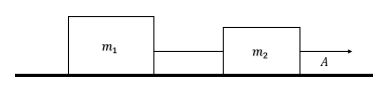
\includegraphics{Sistema de dos bloques amarrados.png}
            \caption{Sistema de dos bloques amarrados}
            \label{fig:Sistema de dos bloques amarrados}
        \end{figure}
        
    Analizando el problema, llegamos al siguiente diagrama de cuerpo libre: 
        
        \begin{figure}[H]
            \centering
            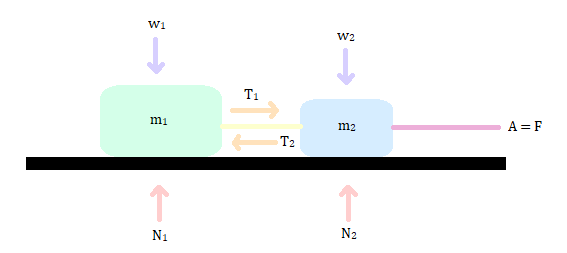
\includegraphics{Diagrama de cuerpo libre de dos bloques amarrados.png}
            \caption{Diagrama de cuerpo libre de un Sistema de dos bloques amarrados}
            \label{fig:Diagrama de cuerpo libre de un Sistema de dos bloques amarrados}
        \end{figure}
        
    Por el diagrama de cuerpo libre notamos que, como el peso de las masas es paralelo a la fuerza normal, es decir, son fuerzas iguales, pero en sentido opuesto, por lo que se cancelan:
    
    \begin{equation}
        \label{Suma de fuerzas n1 y w1}
        N_{1} + w_{1} \thinspace = \thinspace 0
    \end{equation}
    
    \begin{equation}
        \label{Suma de fuerzas n2 y w2}
        N_{2} + w_{2} \thinspace = \thinspace 0
    \end{equation}
    
    Por las ecuaciones \ref{Suma de fuerzas n1 y w1} y \ref{Suma de fuerzas n2 y w2} notamos que esas fuerzas no son necesarias tomarlas en cuenta para el calculo final pues se cancelan entre ellas. \\
    
    Para $m_{1}$, tenemos que, las fuerzas que actuan sobre ella son: 
    
    \begin{equation}
        \label{Fuerzas en m1}
        \vec{T_{1}} \thinspace = \thinspace m_{1} \vec{a}
    \end{equation}
    
    Del mismo modo, notamos que la fuerza $\vec{A}$ actua sobre el bloque de $m_{2}$, por lo tanto, tenemos:
    
    \begin{equation}
        \label{Fuerzas en m2}
        \vec{A} - \vec{T_{2}} \thinspace = \thinspace m_{2} \vec{a}
    \end{equation}
    
    Donde $a$ es la aceleración que experimentan ambos bloques, ya que se mueven a la misma dirección y sentido debido a que están unidos por la cuerda, por lo tanto, al sumas las fuerzas, tenemos que: 
    
    \begin{equation}
        \label{Suma de fuerzas en el sistema}
        \vec{T_{1}} + \vec{A} - \vec{T_{2}} \thinspace = \thinspace m_{1} \vec{a} + m_{2}\vec{a} 
    \end{equation}
    
    Despejando $a$ de la ecuación \ref{Suma de fuerzas en el sistema} tenemos: 
    
    \begin{equation}
        \label{Aceleración del sistema}
        \vec{a} = \frac{\vec{T_{1}} + \vec{A} - \vec{T_{2}}}{m_{1} + m_{2}} 
    \end{equation}
    
    $\therefore$ \thinspace La aceleración del sistema es \ref{Aceleración del sistema} ($\vec{a} = \frac{\vec{T_{1}} + \vec{A} - \vec{T_{2}}}{m_{1} + m_{2}}$) \\
    
    Para calcular la tensión en la cuerda, notemos que, en la imagen \ref{fig:Diagrama de cuerpo libre de un Sistema de dos bloques amarrados} las fuerzas que actuan sobre la cuerda son, la tensión uno ($T_{1}$) y la tensión dos ($T_{1}$), por lo tanto, despejando a $T_{1}$ de \ref{Fuerzas en m1} tenemos:
    
    \begin{equation}
        \label{T1 despejado}
        \vec{T_{1}} \thinspace = \thinspace m_{1} \vec{a}
    \end{equation}
    
    De igual modo, despejando a $T_{2}$ de \ref{Fuerzas en m2} tenemos: 
    
    \begin{equation}
        \label{T2 despejado}
        \vec{T_{2}} \thinspace = \thinspace \vec{A} - m_{1} \vec{a}
    \end{equation}
    
    Por lo tanto, de las ecuaciones \ref{T1 despejado} y \ref{T2 despejado} tenemos para $T$: 
    
    \begin{equation}
        \label{Tensión de la cuerda}
        \vec{T} \thinspace = \thinspace \vec{T_{1}} + \vec{T_{2}} \thinspace = \thinspace \vec{a} \left( m_{1} - m_{2} \right) + \vec{A}
    \end{equation}
    
    $\therefore$ \thinspace La tensión de la cuerda entre los bloques es \ref{Tensión de la cuerda} ($\vec{T} \thinspace = \thinspace \vec{T_{1}} + \vec{T_{2}} \thinspace = \thinspace \vec{a} \left( m_{1} - m_{2} \right) + \vec{A}$) \\
    
\section{Punto Extra}

    \begin{itemize}\renewcommand{\labelitemi}{$\propto$}
        \item Investiguen que hace la paqutería "hyperref" y expliquen que hace, citen su fuente donde fue investigado.\\
    \end{itemize}
    
    Si queremos añadir links a nuestro documento de pdf, para navegar por las diferentes secciones, referencias y citas, podemos usar el paquete {hyperref}, que automaticamente ya añade los links.\\
    
    El paquete hyperref, por hyperref, ($\backslash$usepackage$\{$hyperref$\}$) es usado para tener un control adecuado de todo tipo de links y referencias a lo largo del texto, siendo esto último gracias a que las referencias previas citadas por el comando $\backslash ref$  se convierten automáticamente en links (que al darles click te llevaran directo a dónde está el objeto al que se hace referencia) al momento de aplicar la paquetería en cuestión.\\
    
    Esta paquetería nos da los siguientes comandos nuevos:
    
        \begin{itemize}
            \item $\backslash$url$\{$link$\}$.\\
            
            Este nos permite introducir cualquier link web en su forma  ``real" para hacerle referencia, y al clicar en él ir a la página de este.\\
    
            \item $\backslash$href$\{$link/nombre del archivo local$\}$$\{$nombre con el que aparecera en el texto$\}$ \\
            
            Sirve para lo mismo que el anterior comando, pero tiene la diferencia de que pone el enlace ``oculto" y muestra, en su lugar, una palabra o frase que le atribuyamos; además de que con éste también se puede hacer referencia a archivos locales del documento.\\
    
            \item $\backslash$hyperlink$\{$la palabra/oración$\}$$\{$nombre con el que aparecera en el texto$\}$\\
            
            Sirve para ``enlazar" cualquier palabra del documento a otra parte usando como ``link de referencia" (resaltado de algún color) la palabra que elijamos.\\
    
            \item $\backslash$hypertarget$\{$la palabra/oración$\}$$\{$nombre con el que aparecera en el texto$\}$ \\
            
            En palabras simples, funciona para lo mismo que el anterios comando, pero tiene la diferencia de que no resalta el texto de ningún color.\\
        \end{itemize}
    
\end{enumerate}
     \cite{Cita}
     \printbibliography
     
\end{document}
